\documentclass[c]{beamer}
\usetheme[plain]{NTU}
\usepackage{listings}

\definecolor{lightgrey}{rgb}{0.9,0.9,0.9}
\definecolor{darkgreen}{rgb}{0,0.6,0}

\lstdefinelanguage{BibTeX}
  {keywords={%
      @article,@book,@collectedbook,@conference,@electronic,@ieeetranbstctl,%
      @inbook,@incollectedbook,@incollection,@injournal,@inproceedings,%
      @manual,@mastersthesis,@misc,@patent,@periodical,@phdthesis,@preamble,%
      @proceedings,@standard,@string,@techreport,@unpublished%
      },
   comment=[l][\itshape]{@comment},
   sensitive=false,
}

%\lstset{frame=single,
%        basicstyle=\ttfamily,
%        %identifierstyle=\color{blue}\ttfamily,
%        keywordstyle=\color{red}\ttfamily,
%        stringstyle=\color{black}\ttfamily,
%        commentstyle=\color{green}\ttfamily}

\lstdefinelanguage{MyLaTeX}
{
language=[LaTeX]TeX,
moretexcs={cmdname, subsection,citep,eqref,includegraphics,maketitle,tableofcontents,listoffigures,listoftables},
morekeywords={abstract,article,document,verbatim,equation,figure,table,tabular,envname},
otherkeywords={$, \{, \}, \[, \], \|, \|, \#,-,+,=},
%literate={+}{{{\color{red}+}}}2 {-}{{{\color{red}-{}}}}2 {=}{{{\color{red}=}}}1
}

\lstset{language=MyLaTeX,
frame=single,
texcsstyle=*\bf\color{blue},
numbers=none,
breaklines=true,
basicstyle=\small,
keywordstyle=[1]\bf\color{darkgreen},
%identifierstyle=\textsf,
commentstyle=\color{red},
tabsize=2,
%backgroundcolor=\color{lightgrey}
%breakautoindent=false,
}

%\AtBeginSection{\frame{\sectionpage}}

\AtBeginSection[]
{
  \begin{frame}<beamer>
    \frametitle{Outline for section \thesection}
    \tableofcontents[currentsection]
  \end{frame}
}

\begin{document}

\title{Introduction to \LaTeX}
%\subtitle{Based on Beamer version 3.07}
\author{Tan Wen Jun \\ wtan047@e.ntu.edu.sg}
\institute[NTU]{School of Computer Science and Engineering\\ NTU}
\date{\today}

\begin{frame} %[plain]
  \titlepage
\end{frame}

\begin{frame}{Outline}
  \tableofcontents
  % You might wish to add the option [pausesections]
\end{frame}

\section{Introduction}

\begin{frame}{Why \LaTeX?}
  \begin{itemize}
    \item It makes beautiful Documents
    \begin{itemize}
      \item Especially mathematics and algorithms
    \end{itemize}
    ~
    \item It was created by scientist, for scientist.
    \begin{itemize}
      \item Originally written in 1984 by Leslie Lamport.
    \end{itemize}
    ~
    \item Powerful and Extensible
    \begin{itemize}
      \item Packages for papers, presentations, spreadsheets ...
    \end{itemize}
  \end{itemize}
\end{frame}

\begin{frame}[fragile]{How does it work?}
  \begin{itemize}
    \item \LaTeX{} is a document preparation system for the \TeX{} typesetting program.
    
    \item You write your document in plain text with \emph{commands} that describe its structure and meaning.
    
    \item The \LaTeX{} program processes your text and commands to product a beautifully formatted document.\\
    ~
    \item Example: 
    
\begin{lstlisting}
\emph{Hello} World!
\end{lstlisting}

    \emph{Hello} World!
  \end{itemize}
\end{frame}

\begin{frame}{Different Mindset}
  \begin{itemize}
    \item Use commands to describe `what it is', not `how it looks'.\\
    ~
    \item Focus on your content\\
    ~
    \item Let \LaTeX{} do all the magic
  \end{itemize}
\end{frame}

\begin{frame}{Comparing \LaTeX{} and Word}
\centering
\small
\begin{tabular}{l|p{3.5cm}| p{3.5cm}}
& \LaTeX & Microsoft Word \\ \hline \hline
Paradigm & WYSIWYM    & WYSIWYG \\ \hline
Content  & Plain Text & Formatted Text \\ \hline
Layout   & Automatic  & Manual \\ \hline
%Custom Design   & Difficult  & Easy \\ \hline
Table    & Difficult  & Easy \\ \hline
Equation & In-built   & Equation Editor \\ \hline
Drawing  & TikZ       & Drawing Tools \\ \hline
Spell-check & OpenOffice Dictionary & $\checkmark$ \\ \hline
Grammar-check & LanguageTool & $\checkmark$ \\ \hline
Cross-referencing & Easy & Difficult \\ \hline
Citation & BibTex & EndNote, Mendeley, etc.  \\
%\hline\hline
%Hiding Text & Commenting out & \\ \hline
%Modifications & Diff. changes & Track Changes \\ \hline
%Sharing & Plain text for editing / PDF for reading & Whole Document \\ \hline
%Version Control & Any VCS & Share point \\ \hline
%File Format & Plain Text & XML+Zipped \\ \hline
%OS Support  & Cross-platform & Windows \& Mac OS X 
\end{tabular}
\end{frame}

\begin{frame}{Setting up \LaTeX}
  \begin{itemize}
    \item \TeX~typesetting program
    \begin{itemize}
      \item MiKTeX for Microsoft Windows --  \url{http://www.miktex.org}
      \item MacTeX for Mac OS X -- \url{https://www.tug.org/mactex/}
      \item Tex Live for all OS -- \url{https://www.tug.org/texlive/}
    \end{itemize}
    ~
    \item \LaTeX~Editors
    \begin{itemize}
      \item TexMaker -- \url{http://www.xm1math.net/texmaker/}
      \item TeXstudio -- \url{http://www.texstudio.org}
    \end{itemize}
    ~
    \item Cloud-based Tools
    \begin{itemize}
      \item ShareLatex -- \url{https://www.sharelatex.com}
      \item Overleaf -- \url{https://www.overleaf.com}
    \end{itemize}
    ~
    \item Complete list of Editors --
    \url{https://en.wikipedia.org/wiki/Comparison_of_TeX_editors}
  \end{itemize}
\end{frame}

% % % % % % % % % % % % % % % % % % % % % % % % % % % % % % % % % % % % % % % % % % % % % % % % %
\section{Basics}

\begin{frame}[fragile]{Minimal Document Structure}
\begin{lstlisting}
\documentclass{article}
\begin{document}
Hello World!
\end{document}
\end{lstlisting}

\begin{itemize}
  \item Standard document classes:
  \begin{itemize}
    \item \textbf{article}: for short reports, articles in proceedings or journals, etc.
    \item \textbf{book}: for real books.
  \end{itemize}

  \item Other document classes:
  \begin{itemize}
    \item \textbf{IEEEtran}: IEEE Transactions
    \item \textbf{beamer}: For presentations
  \end{itemize}
\end{itemize}

\end{frame}

\begin{frame}[fragile]{Basics}
\begin{itemize}
\item Commands (0 or more options/arguments)

\begin{lstlisting}
\cmdname[option1, option2...]{arg1}{arg2}
\end{lstlisting}


\item Environments
\begin{lstlisting}
\begin{envname}
environment contents
\end{envname}
\end{lstlisting}


\item Comments: the \% character.
\begin{lstlisting}
% You won't see this line in the output.
You will see this line %<- nothing here!
\end{lstlisting}

\end{itemize}
\end{frame}

\begin{frame}[fragile]{Handling Errors}
\begin{itemize}
\item \LaTeX{} can throw errors when it compiles your document. You need to fix it before it can produce any output.

\item For example, if you misspell \lstinline|\emph| as \verb|\meph|, \LaTeX{} will stop with an ``undefined control sequence'' error.

\item Compile frequently, and fix errors as soon as they arise.

\item If you have just typed caused an error, you can always comment them out and start debugging there.
\end{itemize}
\end{frame}

\begin{frame}[fragile]{Packages}
\begin{itemize}
\item Some commands and environments are built into \LaTeX.

\item \emph{Packages} are libraries of extra commands and environments. There are thousands of freely available packages.

\item We have to load each of the packages we want to use with a \lstinline|\usepackage| command in the \emph{preamble}.
\end{itemize}

\begin{lstlisting}
\documentclass{article}
\usepackage{amsmath} % preamble
\begin{document}
Hello World!
\end{document}
\end{lstlisting}



\end{frame}

\section{Typesetting Text}

\begin{frame}{Whitespace and New Lines}
  \begin{itemize}
    \item Space and tab characters
    \begin{itemize}
      \item White space does not (usually) matter
      \item \TeX determines inter-word spacing to ensure legibility
    \end{itemize}
    ~
    \item Paragraph breaking
    \begin{itemize}
      \item Leave a blank line between text to break paragraph
      \item Multiple blank lines won't give more vertical spacing
      \item \TeX determines inter-line spacing to ensure legibility
    \end{itemize}
    ~
    \item Manual line- and page-breaking?
    \begin{itemize}
      \item TEX decides where to break lines, pages to ensure legibility
      \item if you insist: \textbackslash\textbackslash, \textbackslash pagebreak
    \end{itemize}
  \end{itemize}
\end{frame}


\begin{frame}[fragile]{Effects of Whitespace}
\begin{lstlisting}[basicstyle=\ttfamily\footnotesize]
This is to demonstrate % TODO: comments!
typesetting plain text in \LaTeX. It doesn't care much
about multiple blank spaces and tabs.

``Multiple blank lines'' have the same effect as
one blank line.


Blank lines are for separating paragraphs (content), 
but not how far they are apart (style).
\end{lstlisting}
\begin{center}
\small
\minipage{.5\linewidth}
This is to demonstrate % TODO: comments again!
typesetting plain text in \LaTeX. It doesn't care much about
multiple blank spaces and tabs.

``Multiple blank lines'' have the same effect as one blank line.


Blank lines are for separating paragraphs (content), but not
how far they are apart (style).
\endminipage
\end{center}
\end{frame}

\begin{frame}[fragile]{Quotations}
\begin{itemize}
\item Quotation marks are tricky.
\item Use a backtick (\verb|`|) on the left and an apostrophe (\verb|'|) on the right.
\end{itemize}

\begin{columns}
\begin{column}{0.5\textwidth}
\begin{lstlisting}[basicstyle=\ttfamily\footnotesize]
Single quotes: `text'.

Double quotes: ``text''.
\end{lstlisting}
\end{column}
\begin{column}{0.5\textwidth}
Single quotes: `text'.

Double quotes: ``text''.
\end{column}
\end{columns}

\end{frame}


\begin{frame}[fragile]{Special Characters}
If you just type these characters, you'll get an error.
You have to \emph{escape} it by preceding it with a backslash.
\begin{center}
\begin{tabular}{lll}
\# (hash, pound) & : & \verb|\#| \\
\$ (dollar) & : &  \verb|\$| \\
\% (percent) & : &  \verb|\%| \\
\^{} (``hat'') & : & \verb|\^{}| \\
\& (ampersand) & : & \verb|\&| \\
\_ (underscore) & : & \verb|\_| \\
\{ (left brace) & : & \verb|\{| \\
\} (right brace) & : & \verb|\}| \\
\~{} (tilde) & : & \verb|\~{}| \\
%$\sim$ (wide tilde) & : & \verb|$\sim$| \\
%`` (open double quotes) & : & \verb|``| \\
%'' (close double quotes) & : & \verb|''| \\
\string@ (alias) & : & \verb|\@| \\
\end{tabular}
\end{center}
\end{frame}

\begin{frame}{More Special Characters}
  \begin{itemize}
    \item Mathematical symbols
    ($\alpha$, $\sum$, \dots)
    ~
    \item The Comprehensive \LaTeX Symbol List
    (\url{http://www.texdoc.net/pkg/comprehensive})
    ~
    \item Detexify (\url{http://detexify.kirelabs.org/})
    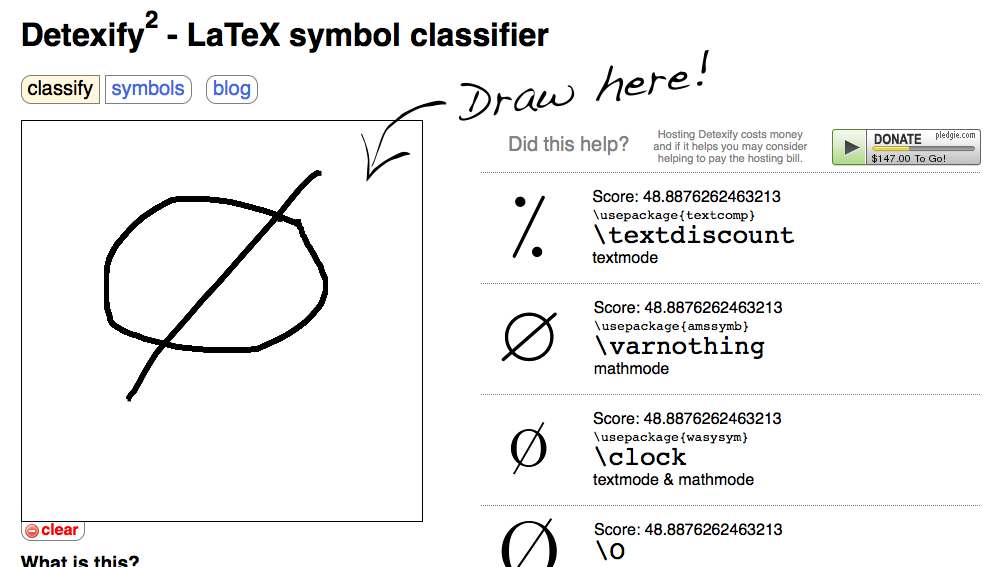
\includegraphics[width=0.6\textwidth]{images/detexify.png}
  \end{itemize}
\end{frame}

\begin{frame}[fragile]{List-Like Environment}
\begin{columns}[onlytextwidth]
  \begin{column}{0.25\textwidth}
    \centering
    Bulleted Lists
\begin{lstlisting}[basicstyle=\ttfamily\scriptsize]
\begin{itemize}
\item one
\item two
\end{itemize}
\end{lstlisting}

\begin{itemize}
  \item one
  \item two
\end{itemize}

  \end{column}
  
  \begin{column}{0.31\textwidth}
    \centering
    Numbered Lists
\begin{lstlisting}[basicstyle=\ttfamily\scriptsize]
\begin{enumerate}
\item one
\item two
\end{enumerate}
\end{lstlisting}
    
    \begin{enumerate}
      \item one
      \item two
    \end{enumerate}
    
  \end{column}
  \begin{column}{0.35\textwidth}
    Description Lists
\begin{lstlisting}[basicstyle=\ttfamily\scriptsize]
\begin{description}
\item[one] is here
\item[two] is there
\end{description}
\end{lstlisting}
    
\begin{description}
  \item[one] is here
  \item[two] is there
\end{description}
    
  \end{column}
\end{columns}
\end{frame}

% % % % % % % % % % % % % % % % % % % % % % % % % % % % % % % % % % % % % % % % % % % % % % % % %
\section{Structuring and Cross-referencing Text}

{
\setbeamertemplate{background canvas}{}
\begin{frame}[fragile]{Sectioning Commands}
  \begin{itemize}
    \item \textbf{article}: \texttt{section}, \texttt{subsection}, \texttt{subsubsection}.
    \item \textbf{book}: \texttt{part} (not usually used), \texttt{chapter}, \texttt{section}, \dots
  \end{itemize}
  
\begin{columns}[onlytextwidth]
  \begin{column}{0.5\textwidth}
\begin{lstlisting}[basicstyle=\ttfamily\footnotesize]
\documentclass{article}

\begin{document}
\section{Introduction}
Introduce your topic here.

\section{Background}
A line or two.

\subsection{Related Work}
Review others' work.

\subsection{Problems}
Unresolved issues.
\end{document}
\end{lstlisting}
  \end{column}
  \begin{column}{0.4\textwidth}
  \textbf{1 Introduction}\\
  Introduce your topic here.\\
  ~
  
  \textbf{2 Background}\\
  A line or two.\\
  ~
  
  \textbf{\small 2.1 Related Work}\\
  Review others' work.\\
  ~
  
  \textbf{\small 2.2 Problems}\\
  Unresolved issues.
  \end{column}
\end{columns}
\end{frame}
}

{
\setbeamertemplate{background canvas}{}
\begin{frame}[fragile]{Cross-referencing}
\begin{itemize}
  \item Bookmark with \verb|\label|,
  \item Reference with \verb|\ref|, \verb|\pageref|
\end{itemize}

\begin{columns}[onlytextwidth]
\begin{column}{0.6\textwidth}
\begin{lstlisting}[basicstyle=\ttfamily\scriptsize]
\documentclass{article}

\begin{document}
\section{Introduction}
\label{sec:intro}
Introduce your topic here.

\section{Background}
\label{sec:background}
Mention section \ref{sec:intro}.

\subsection{Related Work}
\label{sec:related}
Review others’ work.

\subsection{Problems}
\label{sec:problems}
In section \ref{sec:related} on page
\pageref{sec:related}\ldots
\end{document}
\end{lstlisting}
\end{column}
\begin{column}{0.35\textwidth}

\textbf{1 Introduction}\\
Introduce your topic here.\\
~

\textbf{2 Background}\\
Mention section 1.\\
~

\textbf{\small 2.1 Related Work}\\
Review others' work.\\
~

\textbf{\small 2.2 Problems}\\
In section 2.1 on page 1\ldots

\end{column}
\end{columns}
\end{frame}
}



% % % % % % % % % % % % % % % % % % % % % % % % % % % % % % % % % % % % % % % % % % % % % % % % %
\section{Typesetting Mathematics}

\begin{frame}[fragile]{Dollar Signs}
\begin{itemize}
\item \verb|$| are used to mark mathematics in text.
\item Always use dollar signs in pairs -- one to begin the mathematics, and one to end it.
\end{itemize}

\begin{lstlisting}
Let $a$ and $b$ be distinct positive integers,
and let $c = a - b + 1$
\end{lstlisting}

Let $a$ and $b$ be distinct positive integers,
and let $c = a - b + 1$

\end{frame}

\begin{frame}[fragile]{Notations}
\begin{itemize}
\item Use caret (\verb|^|) for superscripts and underscore (\verb|_|) for subscripts.
\begin{tabular}{|l|l|}
\hline
\lstinline|$y = c_2 x^2 + c_1 x + c_0$| & $y = c_2 x^2 + c_1 x + c_0$ \\
\hline
\end{tabular}\\
~
\item Use curly braces \verb|{}| to group subscripts and subscripts.

\begin{tabular}{|l|l|}
\hline
\lstinline|$F_n = F_n-1 + F_n-2$| & $F_n = F_n-1 + F_n-2$ \\
\lstinline|$F_n = F_{n-1} + F_{n-2}$| & $F_n = F_{n-1} + F_{n-2}$ \\
\hline
\end{tabular}\\
~
\item There are commands for Greek letters and common notation

\begin{tabular}{|l|l|}
\hline
\lstinline|$\mu = A e ^{Q/RT}$| & $\mu = A e ^{Q/RT}$ \\
\lstinline|$\Omega = \sum_{k=1}^{n} \omega_k$| & $\Omega = \sum_{k=1}^{n} \omega_k$ \\
\hline
\end{tabular}
\end{itemize}

\end{frame}


\begin{frame}[fragile]{Displayed Equations}
\begin{itemize}
\item For complicated equations, display it on its own line using \lstinline|\begin{equation}| and \lstinline|\end{equation}|.
\end{itemize}

\begin{lstlisting}[basicstyle=\ttfamily\scriptsize]
\eqref{eq:golden:ratio:fibonacci} relates the golden ratio and the Fibonacci series. 

Recall that the golden ratio, 
$\phi = \frac{1}{2} (1 + \sqrt{5})$.

\begin{equation}
\label{eq:golden:ratio:fibonacci}
\phi = 1 + \sum^{\infty}_{n=1}
\frac{ (-1)^{n+1} }{ F_n F_{n+1} }
\end{equation}
\end{lstlisting}

\begin{center}
\small
\minipage{.5\linewidth}
\eqref{eq:golden:ratio:fibonacci} relates the 
golden ratio and the Fibonacci series. 
Recall that the golden ratio, $\phi = \frac{1}{2} (1 + \sqrt{5})$.

\begin{equation}\label{eq:golden:ratio:fibonacci}
\phi = 1 + \sum^{\infty} _{n=1}
\frac{ (-1)^{n+1} }{ F_n F_{n+1} }
\end{equation}
\endminipage
\end{center}

\end{frame}

\begin{frame}[fragile]{More Resource for Writing Mathematics}
  \begin{itemize}
    \item \url{http://en.wikibooks.org/wiki/LaTeX/Mathematics}
    \item \url{http://www.andy-roberts.net/misc/latex/}
    latextutorial9.html, latextutorial10.html
    
    \item Scribble an equation, get the \LaTeX~code:
    \url{http://webdemo.myscript.com/#/demo/equation}
  \end{itemize}
\end{frame}


% % % % % % % % % % % % % % % % % % % % % % % % % % % % % % % % % % % % % % % % % % % % % % % % %
\section{Citations and References}

\begin{frame}[fragile]{BibTeX -- Reference Management Software}
\begin{lstlisting}[language=BibTeX, caption=latex-related.bib]
@ARTICLE{knuth:1984,
author = {Donald E. Knuth},
title = {Literate programming},
journal = {The Computer Journal},
year = {1984},
volume = {27},
number = {2},
pages = {97--111},
address = {Oxford, UK},
publisher = {Oxford University Press}
}
\end{lstlisting}
\end{frame}

\begin{frame}[fragile]{Citing from External .bib File}
\begin{lstlisting}
\documentclass{article}
\begin{document}
\cite{latex:companion} is a useful book. Knuth introduced the literate programming paradigm while developing \TeX{}\ \cite{knuth:1984}.
\bibliographystyle{plain}
\bibliography{latex-related}
\end{document}
\end{lstlisting}
\end{frame}

\begin{frame}{Bibliography Management}
\begin{columns}[t]
\begin{column}{0.4\textwidth}

\begin{itemize}
\item Export references from publishers
  \begin{itemize}
  \item Google Scholar
  \item ScienceDirect
  \item etc.
  \end{itemize}
\item Export from other software
  \begin{itemize}
  \item Mendeley
  \item Zotero
  \item CiteULike
  \item EndNote
  \end{itemize}
\end{itemize}

\end{column}
\begin{column}{0.6\textwidth}
Manage .bib file
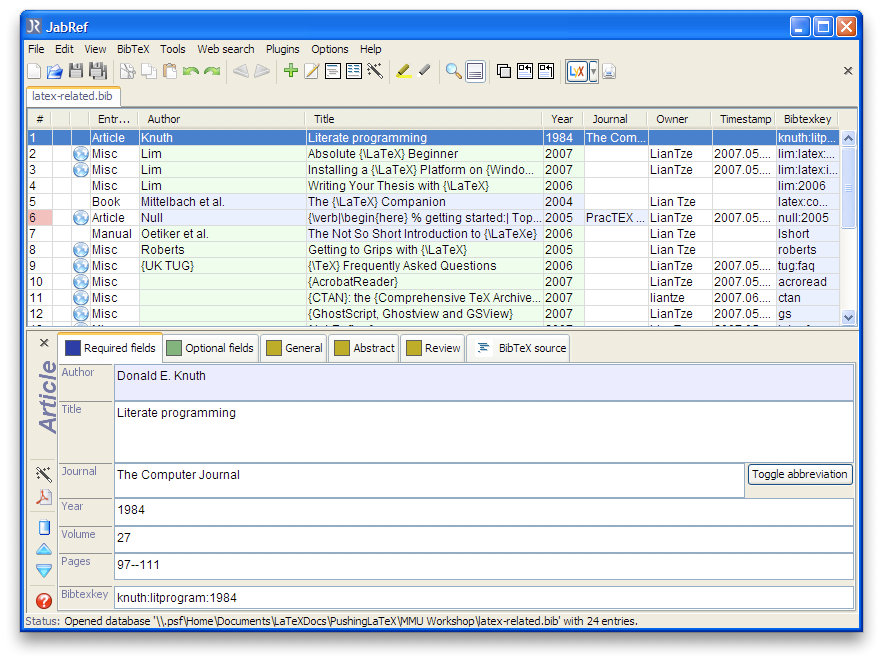
\includegraphics[width=\columnwidth]{images/jabref.png}
\small
\begin{itemize}
\item JabRef: Java-based reference manager\\
\url{http://jabref.sourceforge.net}
\end{itemize}
\end{column}
\end{columns}

\end{frame}


% % % % % % % % % % % % % % % % % % % % % % % % % % % % % % % % % % % % % % % % % % % % % % % % %
\section{Graphics, Figures and Tables}

\begin{frame}[fragile]{Graphics File Format}
\texttt{pdflatex} embeds JPG, PNG and PDF graphic files
\begin{lstlisting}
\usepackage{graphicx}
\includegraphics[width=.3\textwidth]{chick}
\end{lstlisting}

(no file extension $\rightarrow$ automatically looks for \texttt{.jpg}, \texttt{.png}, \texttt{.pdf})

\begin{center}
\includegraphics[width=.2\textwidth]{images/chick}
\end{center}

Other ways to specify the size:\\
\texttt{width=5cm, height=120mm, scale=1.1} ...

\end{frame}


\begin{frame}[fragile]{Figures}
\begin{lstlisting}
\begin{figure}
  \centering
  \includegraphics[width=.3\textwidth]{chick}
  \caption{A chick}
  \label{fig:chick}
\end{figure}
Figure \ref{fig:chick} depicts a chick.
\end{lstlisting}

\begin{figure}
  \centering
  \includegraphics[width=.3\textwidth]{images/chick}
  \caption{A chick}
  \label{fig:chick}
\end{figure}
Figure \ref{fig:chick} depicts a chick.

\end{frame}


\begin{frame}[fragile]{Tabular}
\begin{lstlisting}
\begin{tabular}{|l|c||r|}
  \hline
  one & two two & three three tree \\ \hline
  one one & two two two & three \\ \hline
  one one one & two & three three \\
  \hline \hline
  \multicolumn{2}{|l||}{In the end} & What?! \\
  \hline
\end{tabular}
\end{lstlisting}

\begin{center}
\begin{tabular}{| l | c || r |}
  \hline
  one & two two & three three tree \\ \hline
  one one & two two two & three \\ \hline
  one one one & two & three three \\ \hline\hline
  \multicolumn{2}{|l||}{In the end} & What?! \\ \hline
\end{tabular}
\end{center}
\end{frame}

\begin{frame}{Tabular (Cont.)}
\begin{itemize}
  \item Alternatively, let someone else generate the table for you
  \url{http://www.tablesgenerator.com/}
\end{itemize}
 
\end{frame}

\begin{frame}[fragile]{Tables}
\begin{lstlisting}
\begin{table}
  \centering
  \caption{Sample}\label{tab:sample}
  \begin{tabular}{| l | c || r |}
    \hline
    one & two two & three three tree \\ \hline
    one one & two two two & three \\ \hline
  \end{tabular}
\end{table}

Table \ref{tab:sample} is a very simple example.
\end{lstlisting}

\centering
\begin{table}\centering
  \caption{Sample}\label{tab:sample}
  \begin{tabular}{| l | c || r |}
    \hline
    one & two two & three three tree \\ \hline
    one one & two two two & three \\ \hline
  \end{tabular}
\end{table}
Table \ref{tab:sample} is a very simple example.

\end{frame}

\section*{Misc.}

%\begin{frame}{Additional Resources}
%  \begin{itemize}
%    \item Awesome \LaTeX{}
%    \url{https://github.com/egeerardyn/awesome-LaTeX}
%  
%    \item \LaTeX~on Wikibooks -- excellent tutorial and reference material.
%    \url{https://en.wikibooks.org/wiki/LaTeX}\\
%    
%    \item \TeX~Stack Exchange -- ask questions and get excellent answers.
%    \url{http://tex.stackexchange.com/}
%    
%    \item \LaTeX~Community -- large online forum
%    \url{http://www.latex-community.org/forum/}
%    
%    \item Comprehensive \TeX{} Archive Network (CTAN) -- over 4000 packages plus documentations.
%    \url{http://ctan.org/}
%    
%    \item ShareLaTeX guides 
%    \url{https://www.sharelatex.com/learn/Main_Page}\\
%    
%    \item Online Introduction to Latex from Overleaf\\
%    \href{https://www.overleaf.com/latex/learn/free-online-introduction-to-latex-part-1}{Part 1},
%    \href{https://www.overleaf.com/latex/learn/free-online-introduction-to-latex-part-2}{Part 2}, and 
%    \href{https://www.overleaf.com/latex/learn/free-online-introduction-to-latex-part-3}{Part 3}
%    
%  \end{itemize}
%\end{frame}

\begin{frame}{Other Resources}
  Additional Resources:
  \begin{itemize}
    \item Awesome \LaTeX{}
    \url{https://github.com/egeerardyn/awesome-LaTeX}
  \end{itemize}

  Based on:
  \begin{itemize}
    \item ``Introduction to \LaTeX'' by Lim Lian Tze (Ph.D.), Community TeXpert at Overleaf.
    
    \item Online Introduction to Latex from Overleaf\\
    \href{https://www.overleaf.com/latex/learn/free-online-introduction-to-latex-part-1}{Part 1},
    \href{https://www.overleaf.com/latex/learn/free-online-introduction-to-latex-part-2}{Part 2}, and 
    \href{https://www.overleaf.com/latex/learn/free-online-introduction-to-latex-part-3}{Part 3}
  \end{itemize}
\end{frame}

%%%%%%%%%%%%%%%%%%%%%%%%%%%%%%%%%%%%%%%%%%%%%%%%%%%%%%%%%%%%%%%%%%%%%%%%%%%%%%%
%%%%%%%%%%%%%%%%%%%%%%%%%%%%%%%%%%%%%%%%%%%%%%%%%%%%%%%%%%%%%%%%%%%%%%%%%%%%%%%
%%%%%%%%%%%%%%%%%%%%%%%%%%%%%%%%%%%%%%%%%%%%%%%%%%%%%%%%%%%%%%%%%%%%%%%%%%%%%%%
\begin{frame}
\begin{center}
Thanks, and happy \TeX{}ing!
\end{center}
\end{frame}

\end{document}